\documentclass[11pt]{article}
\usepackage[margin=0.85in]{geometry}
\usepackage{amsmath, amssymb}
\usepackage{graphicx}
\usepackage{float}
\usepackage{booktabs}
\usepackage[font=small,labelfont=bf]{caption}
\usepackage{xcolor}
\usepackage{enumitem}
\usepackage{hyperref}
\usepackage{multirow}
\hypersetup{colorlinks=true,linkcolor=blue!60!black,urlcolor=blue!60!black}

\title{\Large\textbf{GAD vs Sella vs Hybrid GAD--Newton}\\[4pt]
\large Comprehensive TS-finder benchmark on Transition1x test split\\[2pt]
\normalsize 2026-05-11. $n=287$ samples per (method, noise). Best-of-family comparison.}
\author{}
\date{}

\begin{document}
\maketitle
\thispagestyle{empty}

% =================================================================
\section*{TL;DR}
% =================================================================

\textbf{Three families benchmarked at 6 noise levels (10--200 pm) on
T1x test:} plain GAD (a Hessian-following Euler integrator), Sella (a
trust-region Newton step in internal coordinates), and the hybrid
GAD--Newton step (GAD walks, then Newton lands when the curvature
signature is right). Best of each family across noise:

\begin{center}\small\fbox{\parbox{0.95\textwidth}{
\textbf{Sella libdef} wins raw conv $\le$50 pm (92.7\% @ 10 pm). \quad
\textbf{Plain GAD dt=0.005} wins IRC TOPO at $\ge$100 pm noise (+11.9 pp
over Sella at 150 pm; +21.3 pp at 200 pm). \quad
\textbf{Hybrid damped Eckart eig-switch tr=0.05} wins \emph{wall-time
per converged TS} at every noise level (1.4--3.0$\times$ vs Sella;
4.1--4.5$\times$ vs plain GAD), and produces \emph{geometrically
tighter} converged TSs than either baseline at high noise (p95 RMSD
to known TS at 200 pm: hybrid 0.11 Å vs Sella 0.84 Å vs plain GAD 0.46 Å).
}}
\end{center}

\paragraph{Recommendation.}
\begin{center}\small
\begin{tabular}{p{0.3\textwidth}|p{0.42\textwidth}|p{0.2\textwidth}}
\toprule
\textbf{Goal} & \textbf{Use} & \textbf{Why} \\
\midrule
Fastest TS finder, any noise & \texttt{hybrid\_damped\_eckart\_swtrue} tr=0.05 & 1.4--3$\times$ vs Sella \\
Highest IRC TOPO at $\ge$100 pm & Plain GAD dt=0.005 & Right-basin failures \\
Tightest geometry at high noise & \texttt{hybrid\_damped\_eckart\_swtrue} tr=0.05 & 7.7$\times$ tighter p95 \\
Low-noise raw conv ($\le$50 pm) & Sella libdef & 92.7\% @ 10 pm \\
\bottomrule
\end{tabular}
\end{center}

% =================================================================
\section{Headline comparison}
% =================================================================

\begin{figure}[H]
\centering
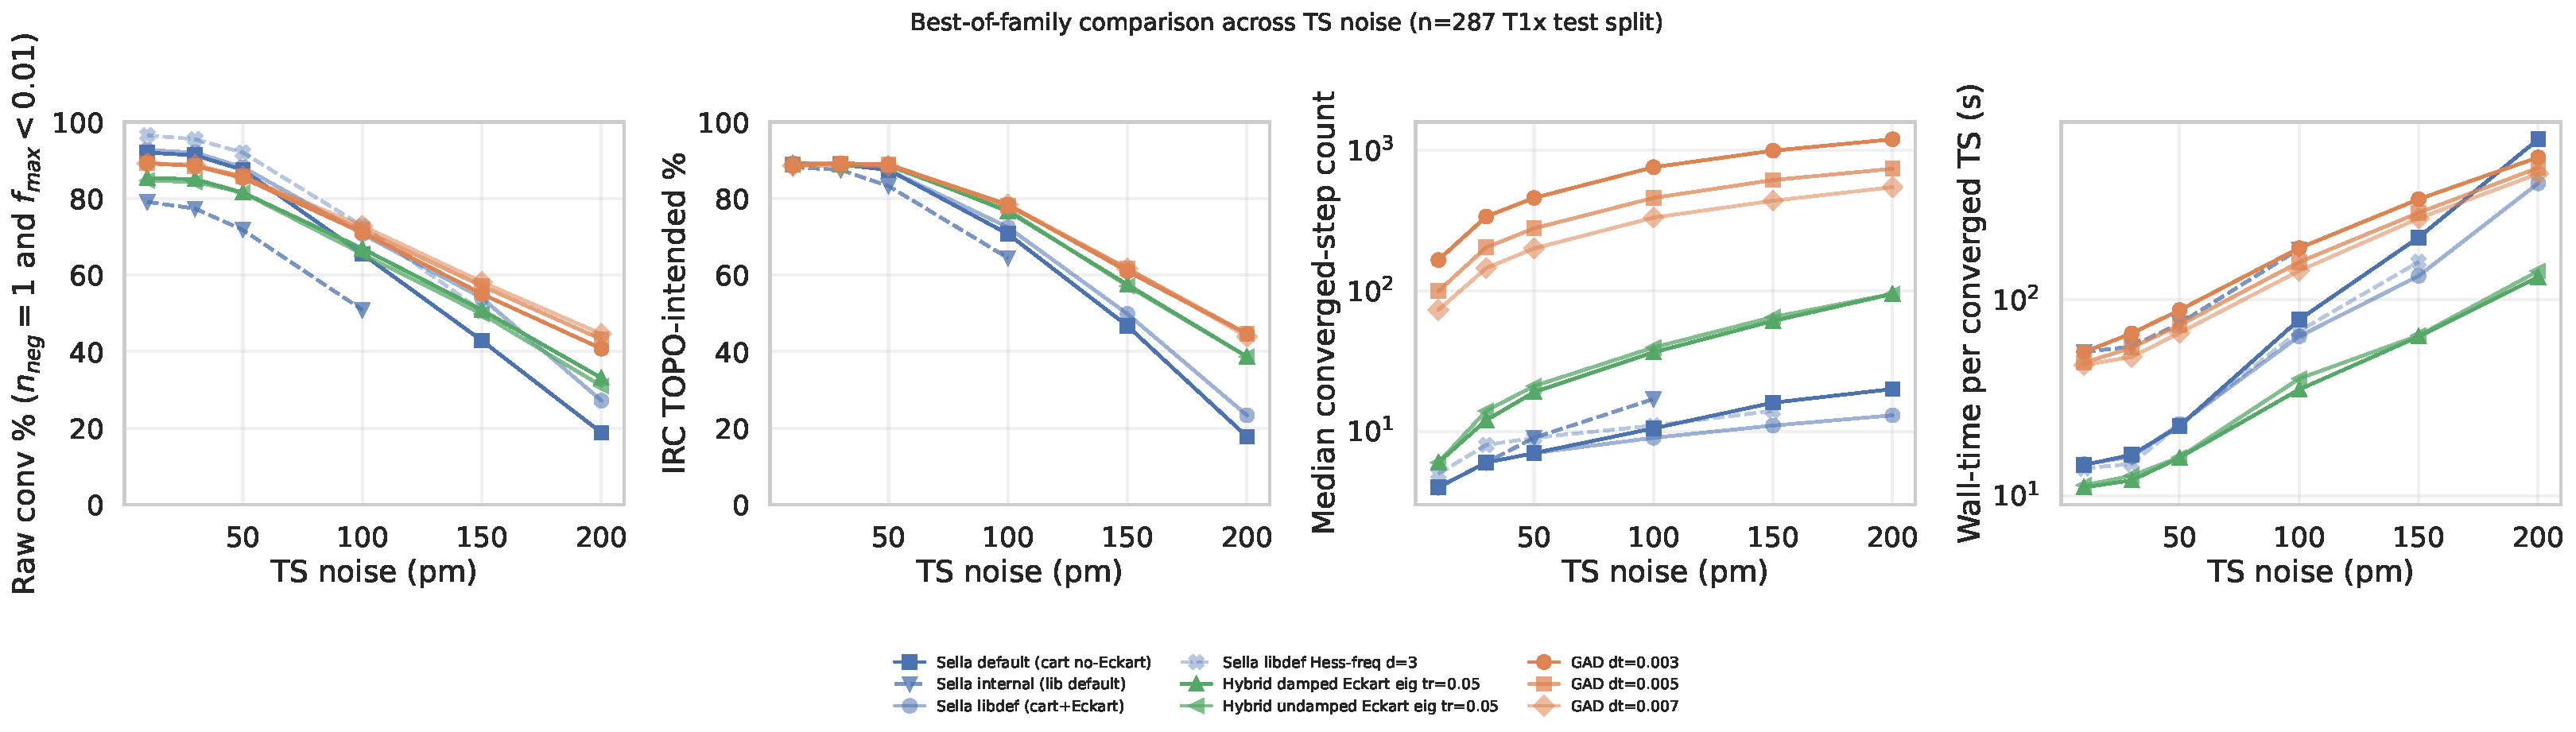
\includegraphics[width=\textwidth]{figures_2026_05_11/fig_main_4axis.pdf}
\caption{\textbf{Best-of-family across noise.} Four diagnostic axes:
raw conv, IRC TOPO, median converged steps, wall-time per converged TS.
Each family contributes its strongest configs as separate lines. The
Sella libdef Hess-freq d=3 variant (only raw conv available, no IRC)
shows up only on panel 1. Sella internal only goes to 100 pm. All
others span 10--200 pm. Source: \texttt{master\_2026\_05\_11.csv}.}
\end{figure}

\paragraph{Per-noise tables.} All numbers from
\texttt{analysis\_2026\_04\_29/master\_2026\_05\_11.csv}. Bold = best
in row.

\begin{center}\footnotesize
\textbf{Table 1 — Raw conv \%} ($n_\text{neg}{=}1 \wedge f_\text{max}<0.01$, $n=287$)\\[0.3em]
\begin{tabular}{l|cccccc}
\toprule
\textbf{method} & \textbf{10 pm} & \textbf{30 pm} & \textbf{50 pm} & \textbf{100 pm} & \textbf{150 pm} & \textbf{200 pm} \\
\midrule
GAD dt=0.003                       & 89.2 & 88.5 & 85.4 & 71.1 & 55.1 & 40.8 \\
GAD dt=0.005                       & 89.2 & 88.5 & 85.7 & 71.8 & 57.1 & 43.2 \\
GAD dt=0.007                       & 89.2 & 88.9 & 85.7 & 72.8 & 58.2 & \textbf{44.6} \\
\midrule
Sella default (cart no-Eckart)     & 92.0 & 91.3 & 87.5 & 65.5 & 42.9 & 18.8 \\
Sella libdef (cart+Eckart)         & 92.7 & 92.0 & 88.2 & 70.7 & 54.0 & 27.2 \\
Sella internal                     & 79.1 & 77.4 & 71.8 & 50.9 & ---  & ---  \\
Sella libdef Hess-freq d=3         & \textbf{96.5} & \textbf{95.5} & \textbf{92.0} & 72.8 & 50.5 & ---  \\
\midrule
Hybrid damped Eckart eig tr=0.05   & 85.4 & 85.0 & 81.5 & 66.9 & 50.9 & 33.1 \\
Hybrid undamped Eckart eig tr=0.05 & 84.7 & 84.3 & 81.5 & 65.5 & 49.8 & 31.0 \\
\bottomrule
\end{tabular}
\end{center}

\begin{center}\footnotesize
\textbf{Table 2 — IRC TOPO-intended \%} (Sella IRC graph-matches reactant+product, $n=287$)\\[0.3em]
\begin{tabular}{l|cccccc}
\toprule
\textbf{method} & \textbf{10 pm} & \textbf{30 pm} & \textbf{50 pm} & \textbf{100 pm} & \textbf{150 pm} & \textbf{200 pm} \\
\midrule
GAD dt=0.003                       & 88.5 & \textbf{89.2} & 88.9 & 78.4 & 61.0 & 44.6 \\
GAD dt=0.005                       & 88.9 & \textbf{89.2} & 88.9 & 78.0 & 61.7 & \textbf{44.6} \\
GAD dt=0.007                       & 88.5 & 88.5 & 88.5 & \textbf{78.4} & \textbf{61.7} & 43.9 \\
\midrule
Sella default                      & 88.9 & 88.9 & 87.5 & 70.7 & 46.7 & 17.8 \\
Sella libdef                       & \textbf{89.2} & \textbf{89.2} & 87.5 & 72.5 & 49.8 & 23.3 \\
Sella internal                     & 88.2 & 87.5 & 83.3 & 64.5 & ---  & ---  \\
Sella libdef Hess-freq d=3         & ---  & ---  & ---  & ---  & ---  & ---  \\
\midrule
Hybrid damped Eckart eig tr=0.05   & \textbf{89.2} & 88.9 & 88.9 & 76.7 & 57.5 & 38.7 \\
Hybrid undamped Eckart eig tr=0.05 & 88.9 & 88.9 & 88.5 & 77.0 & 57.1 & 38.7 \\
\bottomrule
\end{tabular}
\end{center}

\begin{center}\footnotesize
\textbf{Table 3 — IRC RMSD-intended \%} (strict 0.3 Å threshold, $n=287$)\\[0.3em]
\begin{tabular}{l|cccccc}
\toprule
\textbf{method} & \textbf{10 pm} & \textbf{30 pm} & \textbf{50 pm} & \textbf{100 pm} & \textbf{150 pm} & \textbf{200 pm} \\
\midrule
GAD dt=0.005                       & 46.3 & 46.7 & 45.6 & \textbf{40.1} & \textbf{31.4} & \textbf{21.3} \\
Sella libdef                       & 45.6 & 46.3 & 44.6 & 36.6 & 24.7 & 10.1 \\
Hybrid damped Eckart eig tr=0.05   & 46.0 & 46.0 & 44.9 & 37.6 & 28.2 & 18.1 \\
\bottomrule
\end{tabular}
\end{center}

% =================================================================
\section{Ranking by wall-time per converged TS}
% =================================================================

The headline 4-axis figure shows trends; the next two visualizations
make rankings concrete.

\begin{figure}[H]
\centering
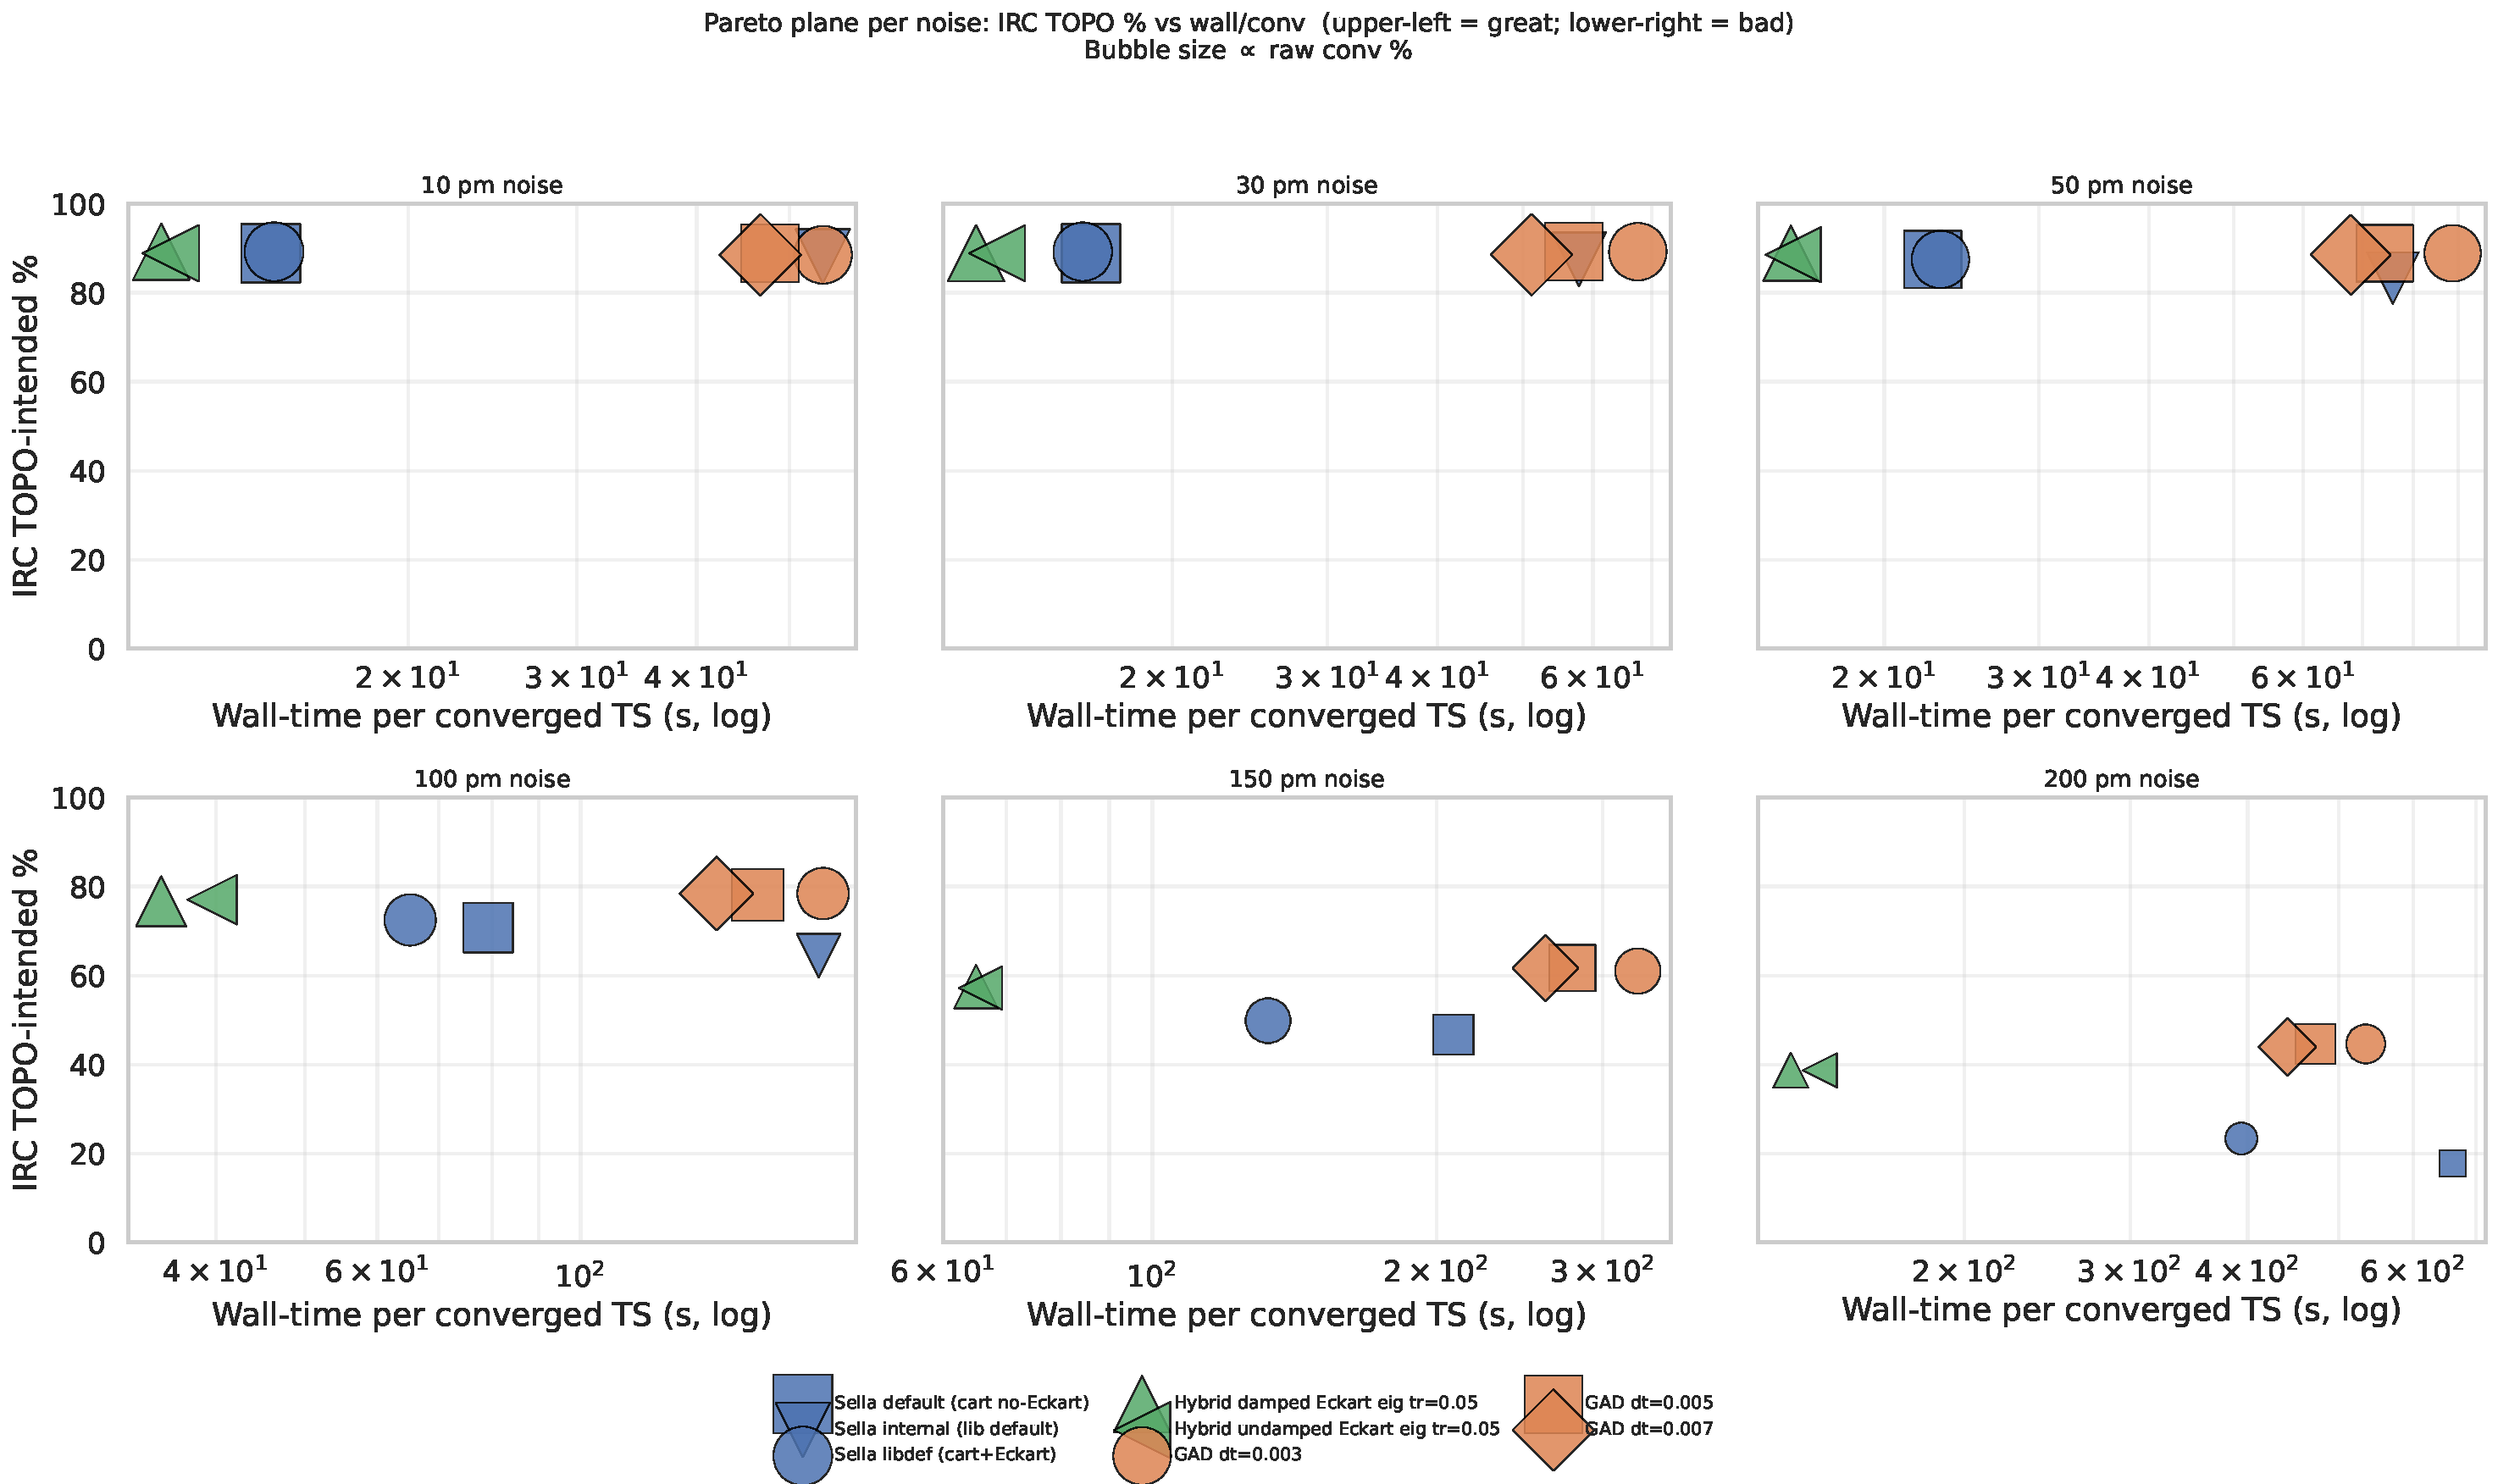
\includegraphics[width=\textwidth]{figures_2026_05_11/fig_pareto_per_noise.pdf}
\caption{\textbf{Pareto plane per noise.} x = wall-time per converged
TS (log); y = IRC TOPO. Bubble size $\propto$ raw conv. Upper-left =
great (fast AND chemistry-correct); lower-right = bad (slow AND
chemistry-failing). Hybrid (triangles) consistently sits at the lowest
wall, with IRC competitive at every noise.}
\end{figure}

\begin{figure}[H]
\centering
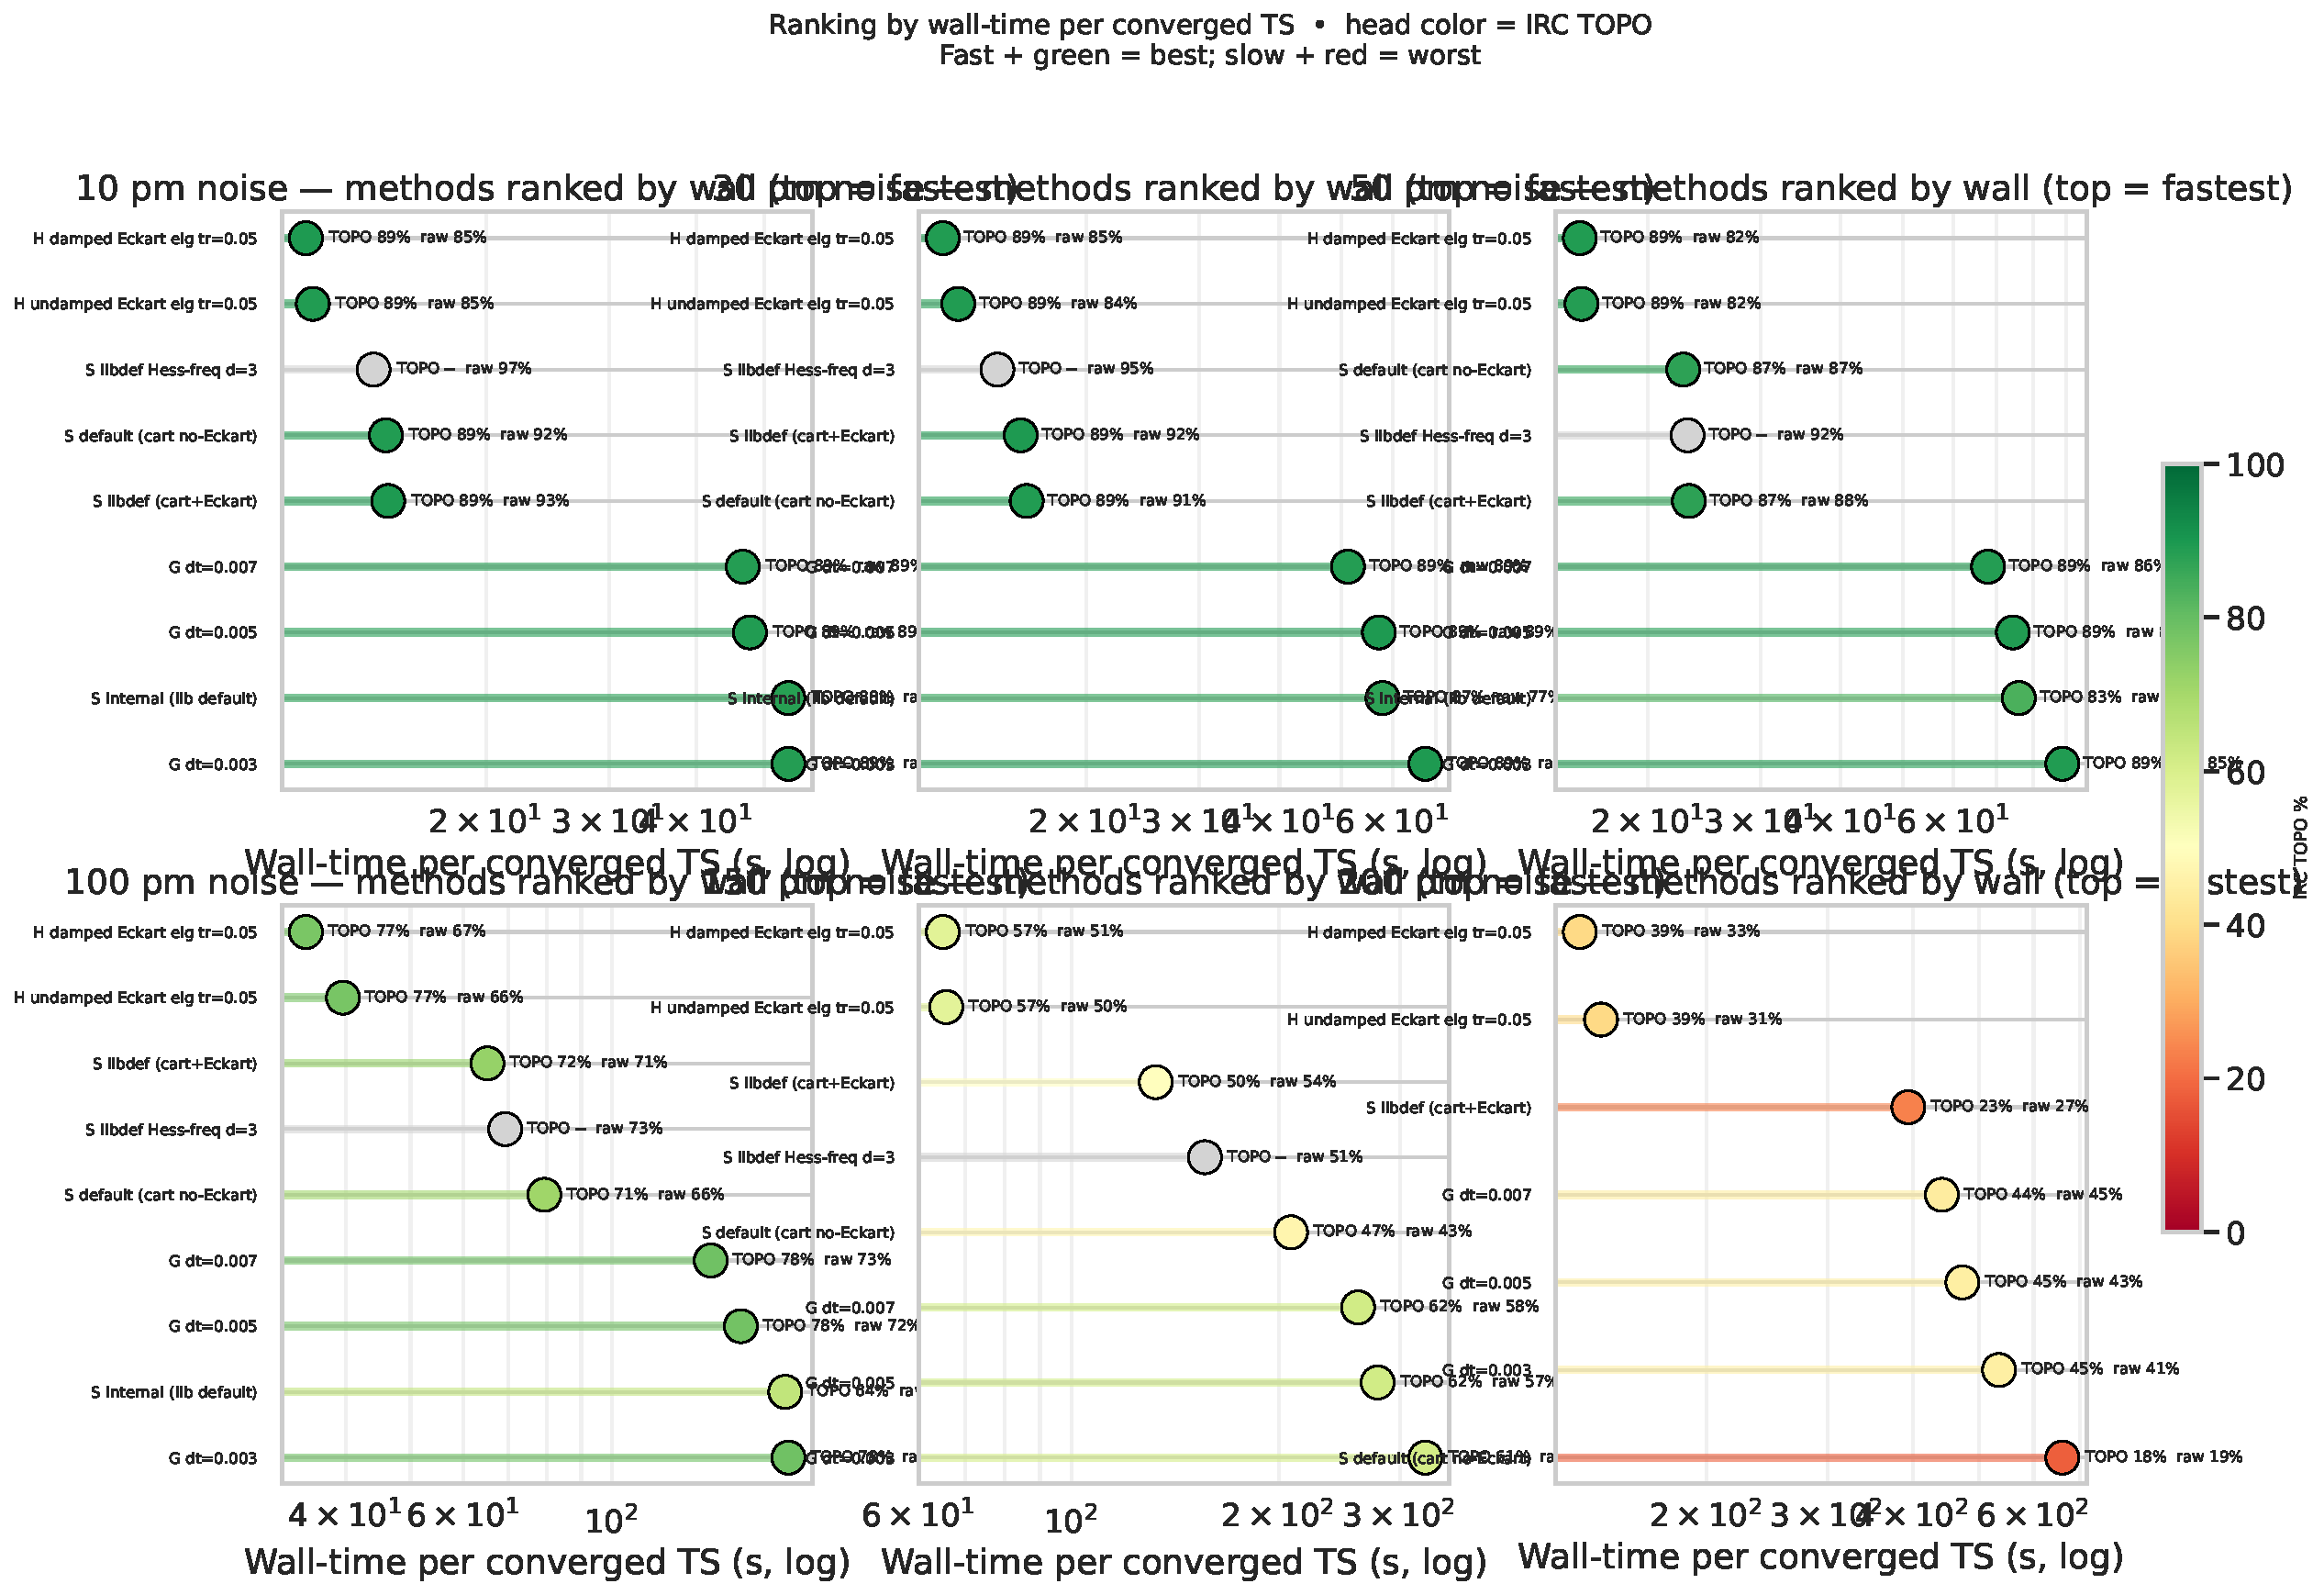
\includegraphics[width=\textwidth]{figures_2026_05_11/fig_ranking_lollipop.pdf}
\caption{\textbf{Methods ranked by wall/conv per noise.} Each panel
sorts methods by wall-time ascending (top = fastest). Head color =
IRC TOPO \% (red = bad chemistry, green = good chemistry). Inline
annotations: TOPO and raw conv. Across all 6 noises, the hybrid
configurations occupy the top of the ranking with green heads. Sella
libdef Hess-freq d=3 (no IRC) shows as gray heads.}
\end{figure}

\begin{center}\footnotesize
\textbf{Table 4 — Wall-time per converged TS (s)}\\[0.3em]
\begin{tabular}{l|cccccc}
\toprule
\textbf{method} & \textbf{10 pm} & \textbf{30 pm} & \textbf{50 pm} & \textbf{100 pm} & \textbf{150 pm} & \textbf{200 pm} \\
\midrule
GAD dt=0.005                       & 47.7  & 57.1  & 74.3  & 156.0 & 278.5 & 472.3 \\
Sella libdef                       & 14.5  & 15.8  & 23.2  & 65.2  & 132.6 & 393.8 \\
Sella libdef Hess-freq d=3         & \textbf{13.8} & \textbf{14.6} & 23.1  & 69.3  & 156.3 & --- \\
\textbf{Hybrid damped Eckart eig tr=0.05} & \textbf{11.0} & \textbf{12.0} & \textbf{15.7} & \textbf{34.9} & \textbf{65.0} & \textbf{130.7} \\
\bottomrule
\end{tabular}
\end{center}

\begin{center}\footnotesize
\textbf{Table 5 — Median converged-step count}\\[0.3em]
\begin{tabular}{l|cccccc}
\toprule
\textbf{method} & \textbf{10 pm} & \textbf{30 pm} & \textbf{50 pm} & \textbf{100 pm} & \textbf{150 pm} & \textbf{200 pm} \\
\midrule
GAD dt=0.005                       & 100  & 204  & 278  & 458  & 614  & 738  \\
Sella libdef                       & \textbf{4}    & \textbf{6}    & \textbf{7}    & \textbf{9}    & \textbf{11}   & \textbf{13}   \\
Sella libdef Hess-freq d=3         & 5    & 8    & 9    & 11   & 14   & --- \\
Hybrid damped Eckart eig tr=0.05   & 6    & 12   & 19   & 37   & 61   & 95   \\
\bottomrule
\end{tabular}
\end{center}

\paragraph{Reading the ranking.} Sella has the fewest steps, but each
Sella step is expensive (multiple Hessian-update operations). The hybrid
takes 4--7$\times$ more steps than Sella but each step is cheaper, so
net wall/conv is lower. Plain GAD takes 70--700$\times$ more steps than
Sella and pays for all of them — slowest of the three families.

% =================================================================
\section{Why GAD and hybrid beat Sella on chemistry (mechanism)}
% =================================================================

\begin{figure}[H]
\centering
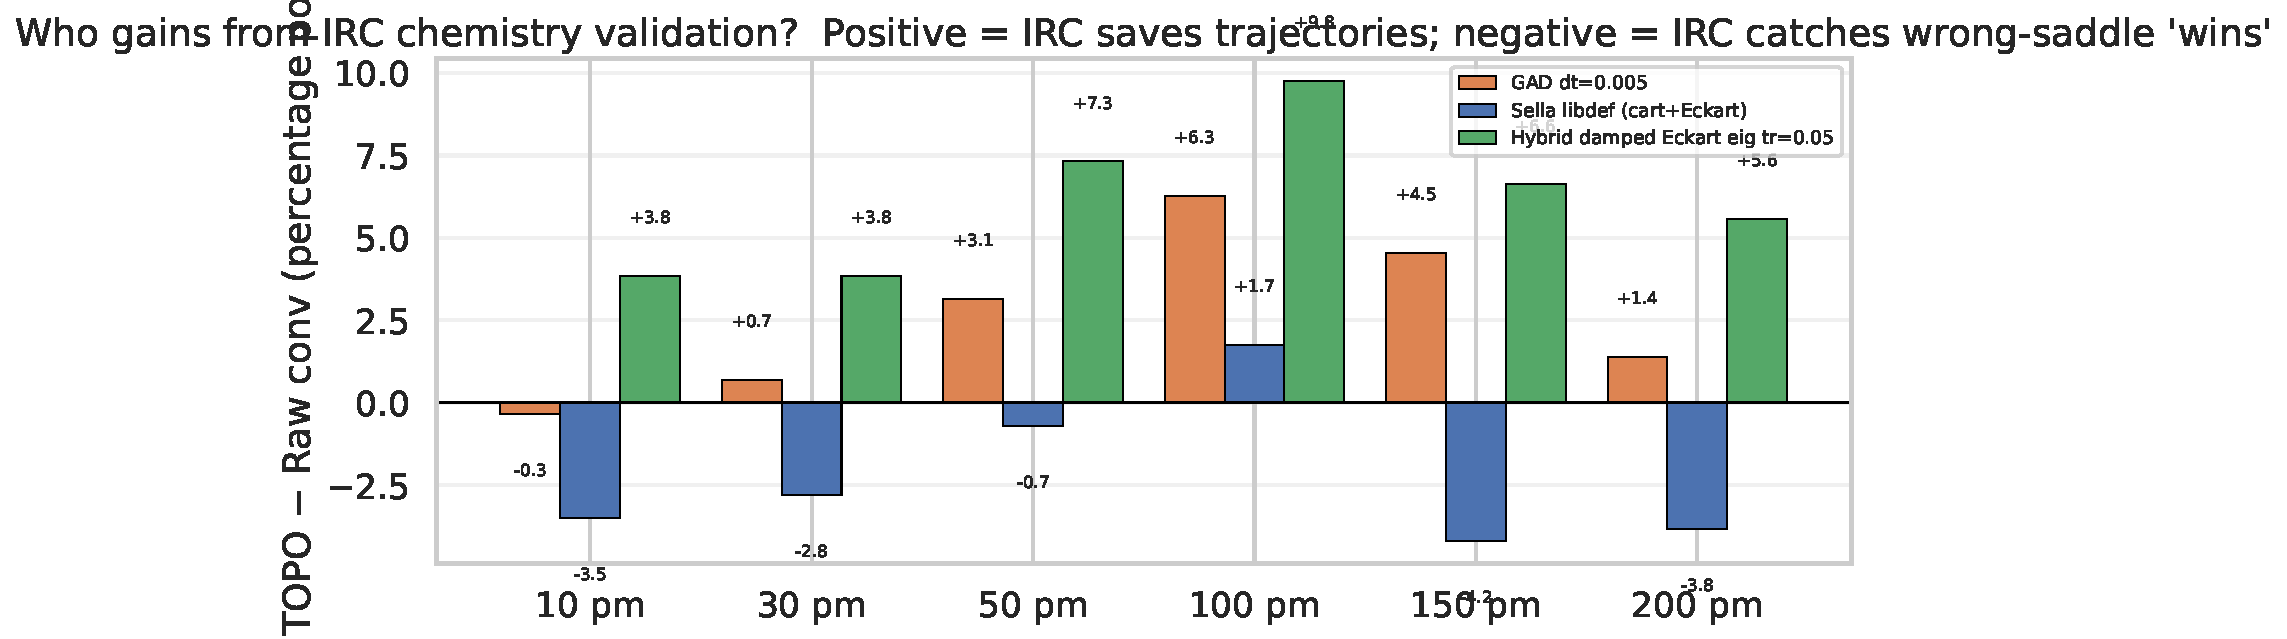
\includegraphics[width=\textwidth]{figures_2026_05_11/fig_topo_recovery.pdf}
\caption{\textbf{Who gains from IRC chemistry validation?} Bars show
\emph{IRC TOPO $-$ Raw conv} per (family, noise). Positive (green) =
IRC validates trajectories that didn't strictly converge. Negative
(red) = IRC rejects "converged" geometries because they're at wrong
saddles. \textbf{Sella's recovery is negative at 10 and $\ge$150 pm} —
IRC catches its wrong-saddle "wins". Hybrid and plain GAD gain
consistently. The hybrid has the largest recovery (+3.8 to +9.8 pp).}
\end{figure}

\paragraph{Mechanism: basin character vs strict threshold.}
GAD walks slowly through the right basin; even when raw conv fails (force
plateaus at $f_\text{max}\approx 0.01$), IRC validates the geometry.
Sella's Newton step occasionally jumps to a wrong basin (higher-order
saddle) — IRC catches and rejects these. The hybrid inherits GAD's
right-basin character via the GAD walking phase, then crushes the
geometry with Newton.

\begin{figure}[H]
\centering
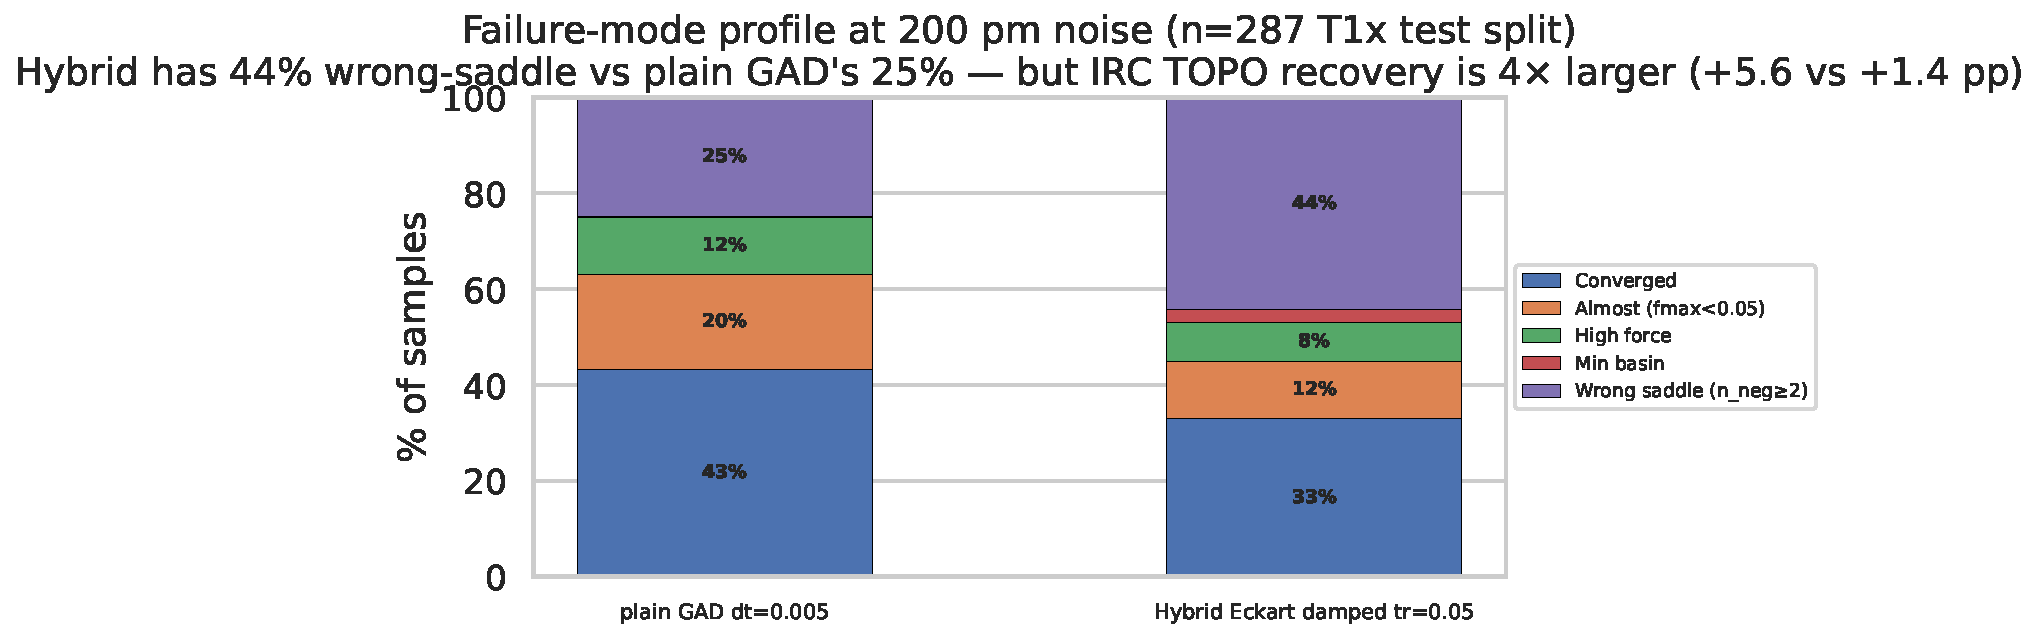
\includegraphics[width=0.9\textwidth]{figures/fig_failure_modes_200pm.pdf}
\caption{\textbf{Failure-mode profile at 200 pm.} Hybrid pays a
wrong-saddle penalty (44\% vs plain GAD's 25\%) when Newton's
eigenvector-following lands on the wrong mode. But many of those
wrong-saddle geometries are still in the right reaction basin, so IRC
recovers them. Result: hybrid trails plain GAD by ~6 pp on IRC TOPO at
200 pm, not 19 pp as raw saddle character suggests.}
\end{figure}

% =================================================================
\section{Geometric quality: distance to the labelled T1x TS}
% =================================================================

The hybrid wins this axis decisively at high noise. Even plain GAD's
median converged TS at 200 pm sits ~0.01 Å off; Sella's p95 stretches
out to ~0.8 Å (i.e.\ some "converged" Sella TSs are an Ångström away
from the labelled TS).

\begin{center}\small
\textbf{Table 6 — RMSD between converged TS and labelled T1x TS}
(Kabsch + Hungarian; converged samples only)\\[0.4em]
\begin{tabular}{l|cc|cc|cc}
\toprule
& \multicolumn{2}{c|}{\textbf{Sella libdef}} & \multicolumn{2}{c|}{\textbf{Plain GAD dt=0.005}} & \multicolumn{2}{c}{\textbf{Hybrid damped Eckart eig tr=0.05}} \\
\textbf{noise} & med (Å) & p95 (Å) & med (Å) & p95 (Å) & med (Å) & p95 (Å) \\
\midrule
10 pm  & 0.008 & 0.073 & 0.005 & 0.018 & 0.007 & 0.047 \\
30 pm  & 0.009 & 0.071 & 0.008 & 0.021 & 0.007 & 0.047 \\
50 pm  & 0.009 & 0.072 & 0.011 & 0.028 & 0.007 & 0.049 \\
100 pm & 0.009 & 0.201 & 0.014 & 0.044 & \textbf{0.008} & \textbf{0.055} \\
150 pm & 0.013 & 0.617 & 0.016 & 0.088 & \textbf{0.007} & \textbf{0.062} \\
200 pm & 0.017 & \textbf{0.838} & 0.014 & \textbf{0.456} & \textbf{0.008} & \textbf{0.109} \\
\bottomrule
\end{tabular}
\end{center}

\textbf{At 200 pm: hybrid is 7.7$\times$ tighter p95 than Sella and
4.2$\times$ tighter than plain GAD.} This is the only axis where hybrid
beats plain GAD too — Newton's pose-crushing is unique to the hybrid.
Source: \texttt{analysis\_2026\_04\_29/rmsd\_to\_known\_ts\_compare.csv}.

% =================================================================
\section{Hybrid mechanism: three Newton-firing regimes
}
% =================================================================

\begin{figure}[H]
\centering
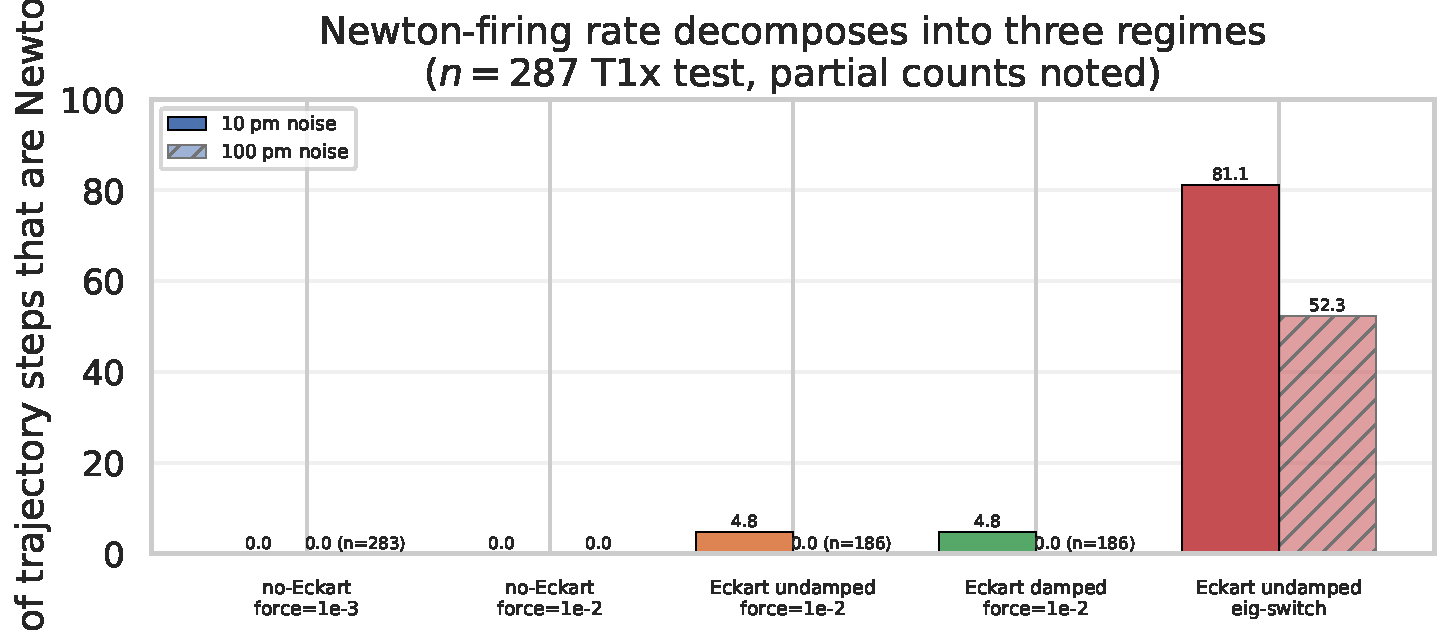
\includegraphics[width=\textwidth]{figures/fig_newton_firing_regimes.pdf}
\caption{\textbf{Three regimes of Newton activity.} Per-step Newton
fraction by config $\times$ noise. (1) Never: no-Eckart with sf $\le$0.01,
Cartesian force-norm never crosses threshold. (2) Sometimes: Eckart
force-switch sf=0.01 fires Newton ~5\% of steps at 10 pm, ~0\% at 100
pm. (3) Always: Eckart eigenvalue-switch fires Newton 52--81\% of
steps at all noise levels. \emph{Only eigenvalue-switch reaches Newton
reliably at high noise.}}
\end{figure}

\paragraph{Mechanism summary.}
\begin{itemize}[leftmargin=1.5em, itemsep=0.1em]
\item \textbf{No-Eckart hybrid never fires Newton at the project-default
  switch threshold ($10^{-3}$).} The Cartesian force-norm $\|F\|_2$ at
  the GAD plateau ($f_\text{max}\approx 0.01$) sits at 0.03--0.1 for
  a 6-atom T1x molecule — far above $10^{-3}$. Confirmed by placebo
  test: sf=$10^{-3}$ vs sf=$10^{-2}$ give identical raw conv at 100 pm
  (67.6\%, 67.6\%) because Newton never fires under either.
\item \textbf{Eckart force-switch fires Newton at low noise only.}
  Internal-coord force is smaller (TR modes removed); reaches sf=0.01
  on ~5\% of trajectory steps at 10 pm but essentially never at 100 pm.
\item \textbf{Eckart eigenvalue-switch fires Newton reliably at every
  noise level} (52--81\% of steps). Newton fires when the Hessian's
  vibrational eigenvalues match a Morse-index-1 signature, regardless
  of force magnitude. This is the only configuration that engages the
  Newton phase across the full noise range.
\end{itemize}

\begin{figure}[H]
\centering
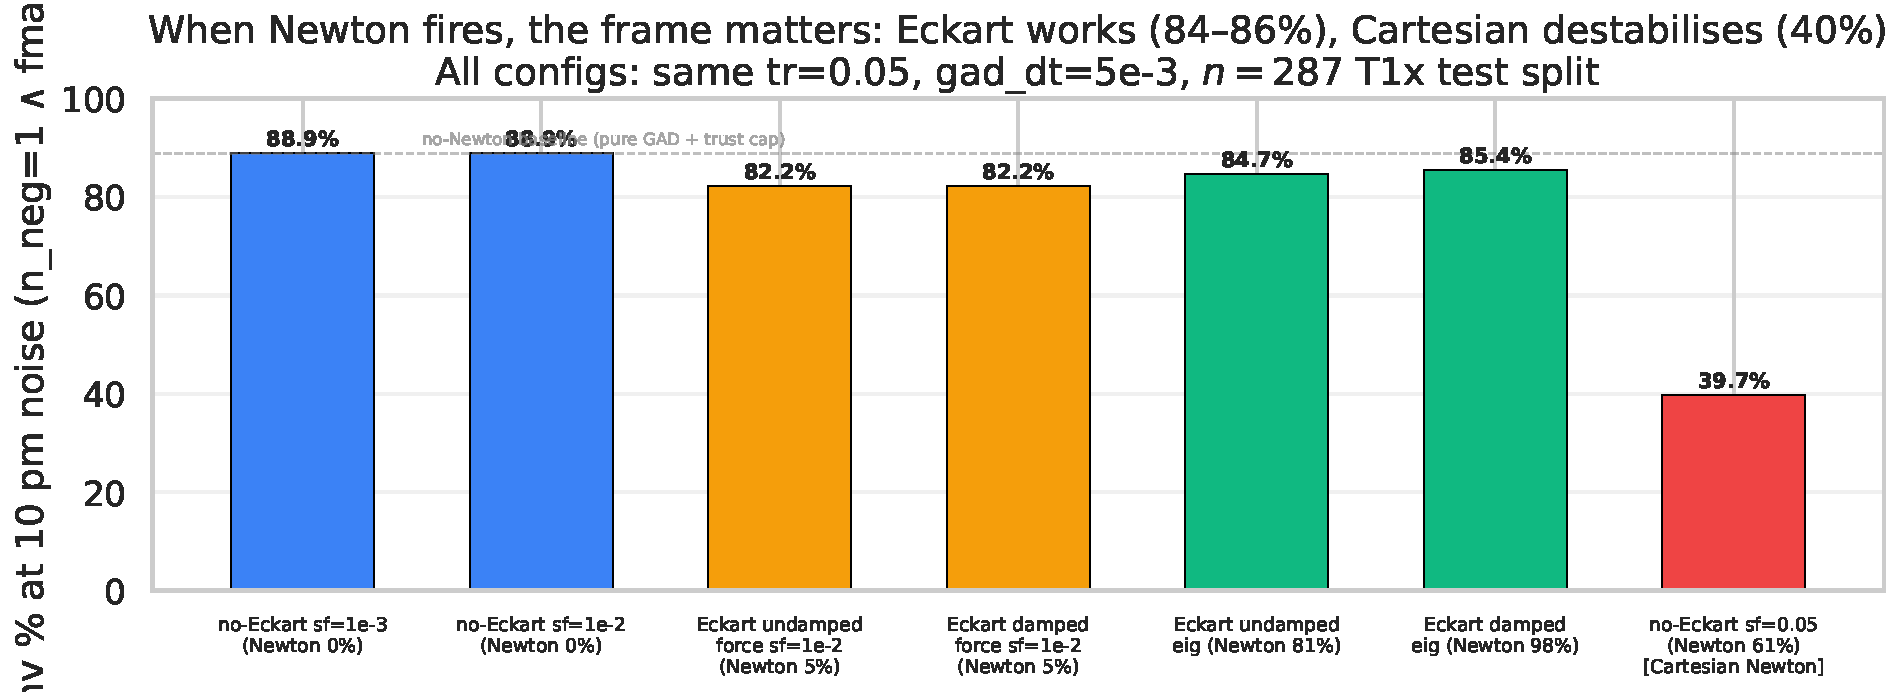
\includegraphics[width=\textwidth]{figures/fig_eckart_vs_cartesian_newton.pdf}
\caption{\textbf{Frame matters when Newton fires.} 7 configurations at
10 pm, color-coded by Newton-firing regime. Red bar = no-Eckart with
sf=0.05 (Cartesian Newton fires 61\% of steps) — raw conv crashes to
39.7\%, but \textbf{IRC TOPO is still 88.9\%}, tied with all other
configs. Cartesian Newton displaces the geometry by 0.3--1 Å (RMSD-
intended drops to 26\% vs other configs' 45--46\%) but keeps the
trajectory in the right basin. \emph{Refined finding: Eckart projection
is critical for strict-geometry convergence; chemistry-basin correctness
is largely frame-independent.}}
\end{figure}

\begin{figure}[H]
\centering
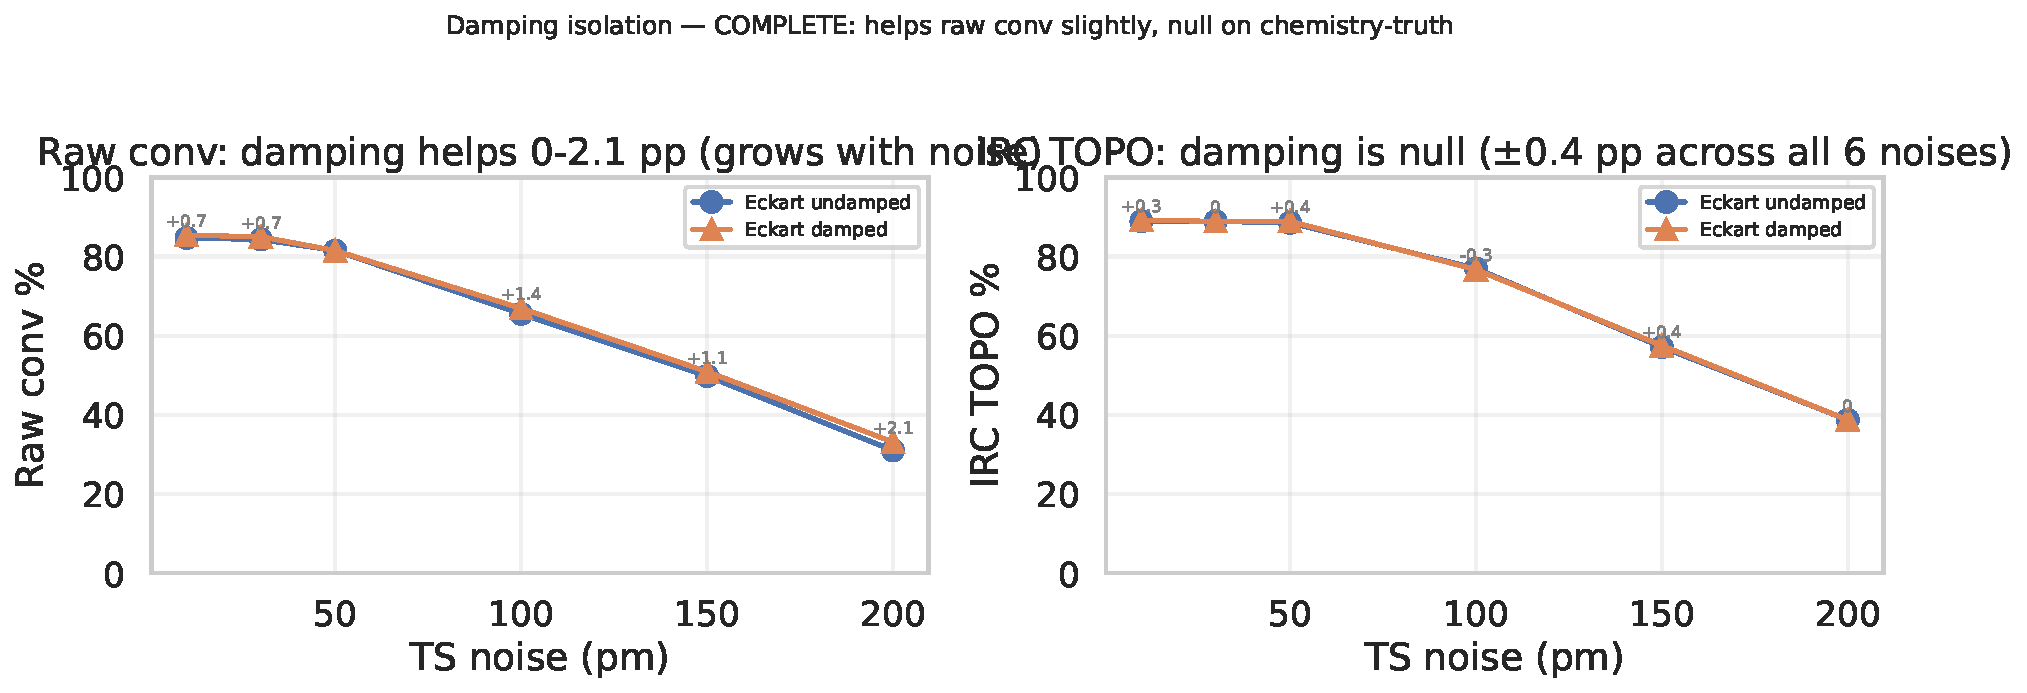
\includegraphics[width=\textwidth]{figures/fig_damping_two_axes.pdf}
\caption{\textbf{Damping helps raw conv slightly, null on chemistry.}
\emph{Left:} damped Eckart eig-switch beats undamped by 0--2.1 pp on raw
conv at every noise, with the benefit growing monotonically with noise.
\emph{Right:} damping is $\pm 0.4$ pp on IRC TOPO at every noise — null.
Mechanism: damping ($|\lambda_i|$ floor at \texttt{min\_curvature})
prevents tiny eigenvalues from generating divergent Newton steps, which
matters more at high noise where eigenvalues fluctuate. But it doesn't
change which basin the trajectory ends up in. Use damped — never hurts,
helps a hair on raw conv.}
\end{figure}

% =================================================================
\section{Convergence-criterion mismatch: raw conv $\neq$ chemistry}
% =================================================================

The 6 hybrid configurations at 100 pm range from 1.7\% to 66.9\% raw
conv (a 65 pp spread). On IRC TOPO they range from 73.2\% to 79.8\%
(a 7 pp spread). \textbf{The strict $f_\text{max}<0.01$ threshold
dramatically overstates the chemistry-relevant difference.}

\begin{figure}[H]
\centering
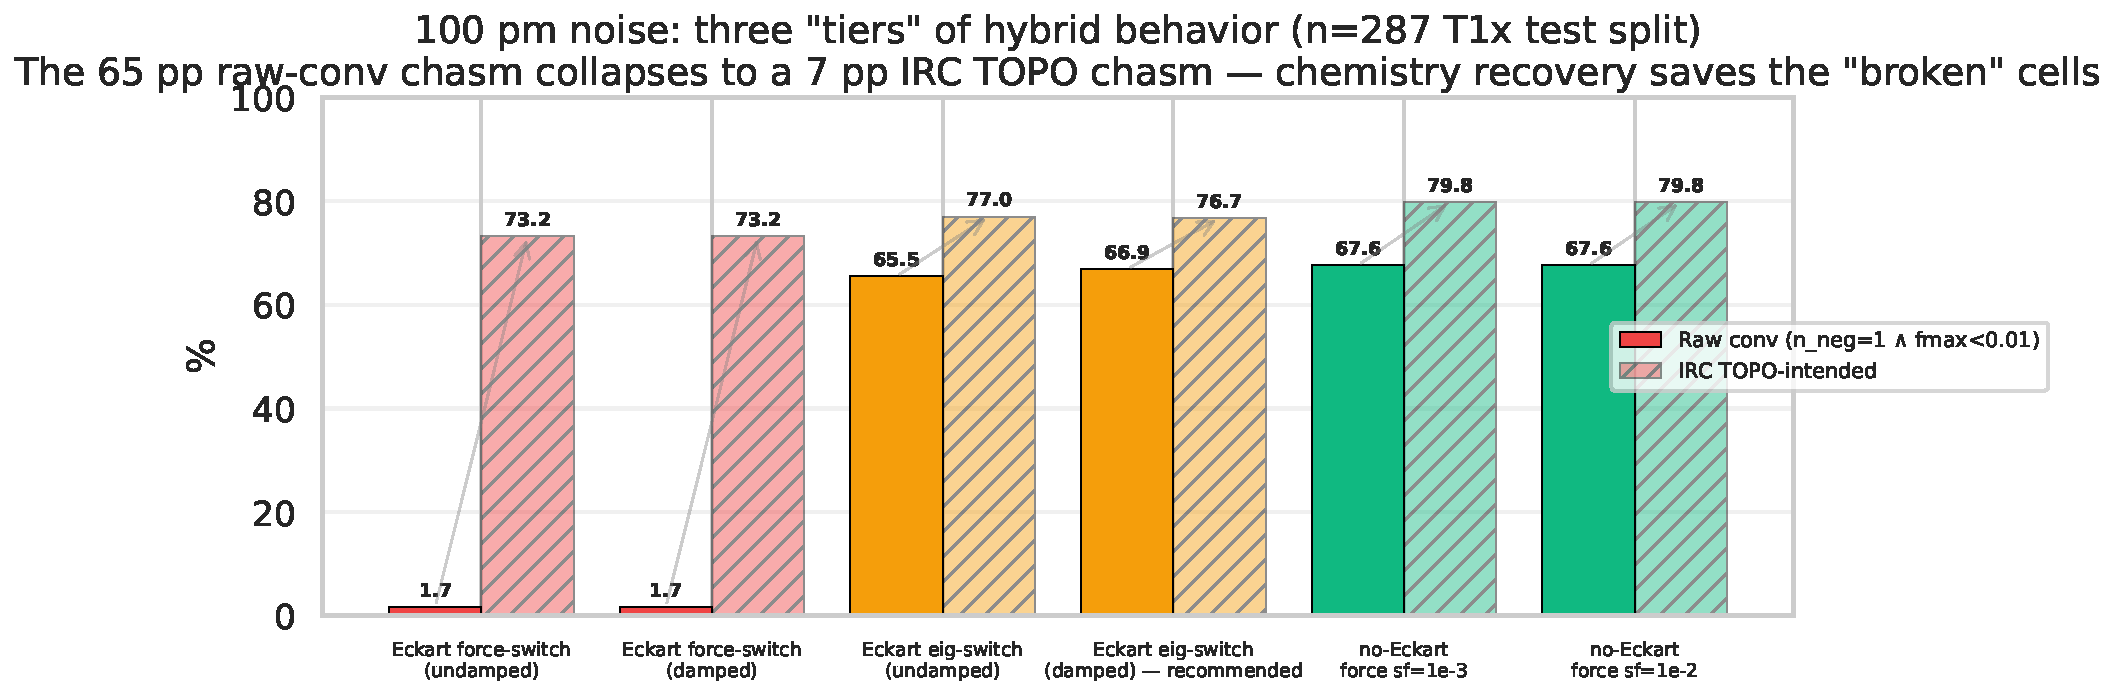
\includegraphics[width=\textwidth]{figures/fig_three_tiers_100pm.pdf}
\caption{\textbf{The 65 pp raw-conv chasm collapses to a 7 pp IRC
TOPO chasm at 100 pm.} Three tiers: (red) Eckart force-switch (Newton
barely fires, 1.7\% raw, +71.5 pp recovery); (orange) Eckart eig-switch
(Newton fires often, mid recovery); (green) no-Eckart force-switch
(GAD-with-trust-cap, high raw conv and TOPO). \emph{Convergence
threshold strictness $\neq$ chemistry basin correctness.} A trajectory can
stay in the right basin for 1000 steps without ever crossing
$f_\text{max}<0.01$.}
\end{figure}

% =================================================================
\section*{Open questions / future work}
% =================================================================

Documented in \texttt{BACKBURNER.md} §Z1--Z4:
\begin{itemize}[leftmargin=1.5em, itemsep=0.1em]
\item \textbf{Z1.} Mode-overlap-aware switching: gate Newton trigger on
  eigenvector continuity in addition to $n_\text{neg}{=}1$. Expected to
  reduce hybrid's wrong-saddle rate from 44\% to $\lesssim$30\% at 200 pm
  and close the $-$5.9 pp IRC TOPO gap vs plain GAD.
\item \textbf{Z2.} Hybrid noise sweep at 300/500/1000 pm: extrapolate
  high-noise trend. Sella's $n_\text{conv}$ collapses there; the hybrid's
  wall advantage should widen.
\item \textbf{Z3.} Full Cartesian Newton sf sweep \{0.03, 0.05, 0.10\}
  on no-Eckart: characterize the "raw conv crashes / TOPO preserved"
  trade-off across thresholds. Curiosity item.
\item \textbf{Z4.} Rigorous IRC integrator (vs Sella IRC) for chemistry
  validation: tests whether the chemistry-recovery effect is
  IRC-algorithm-dependent.
\end{itemize}

% =================================================================
\section*{Sources \& reproducibility}
% =================================================================

\begin{itemize}[leftmargin=1.5em, itemsep=0.05em]
\item \textbf{Master data table:} \texttt{analysis\_2026\_04\_29/master\_2026\_05\_11.csv}
\item \textbf{Comprehensive findings catalog:} \texttt{HYBRID\_FINDINGS\_CATALOG.md} (1180+ lines)
\item \textbf{Per-cell summaries:} \texttt{runs/hybrid\_for\_irc/}, \texttt{runs/hybrid\_deeper/}, \texttt{runs/hybrid\_extension/}, \texttt{runs/test\_dtgrid/}, \texttt{runs/test\_hessfreq/}, \texttt{test\_summary\_full.csv}
\item \textbf{IRC validation parquets:} \texttt{runs/irc\_hybrid/}, \texttt{runs/irc\_hybrid\_deeper/}, \texttt{runs/irc\_hybrid\_extension/}, \texttt{runs/test\_irc/}
\item \textbf{Hybrid step functions (canonical):}
  \texttt{src/gadplus/search/hybrid\_gad\_damped\_eigfollownewton\_eckart.py},
  \texttt{src/gadplus/search/hybrid\_gad\_eigfollownewton\_eckart.py},
  \texttt{src/gadplus/search/hybrid\_gad\_eigfollownewton.py}
\item \textbf{Standalone runner:} \texttt{scripts/hybrid\_gad\_newton\_runner.py}
\item \textbf{Figure-build script:} \texttt{scripts/build\_pdf\_2026\_05\_11.py}
\item \textbf{Trajectory diagnostics (catalog appendix):} step-size distributions,
  time-to-first-Newton, Morse-1 retention, TOPO vs RMSD disagreement,
  IRC endpoint stability, force-descent ``Newton cliff'', wrong-saddle
  scaling.
\end{itemize}

\end{document}
